\chapter{Host Compiled Simulation}

Host Compiled Simulation (HCS) is a popular research topic as a techniques to accelerate the benchmarking of processors. \gls{hcs} is based on the approach of Source Code Instrumentation (SCI). Instrumentation is the technique to modify the source code of an application, in order to extract debug or trace information at run-time. In \gls{hcs}, the source code is instrumented to estimate the time spent in executing the application on a particular target processor. The instrumented source code is run on the host machine, and hence the name.

While earlier research has mostly focussed on using \gls{hcs} for timing estimation, in this work the technique has been extended to estimate the power consumption.

When an application is run on a processor, most of the time is spent in following phases.

\begin{itemize} \itemsep -6pt
\item Execution of instructions.
\item Fetching Data from memory.
\end{itemize}

The technique is based on the assumption, that number of cycles spent in each phase of the execution can be accurately predicted using instrumentation. The trace generated from the run-time can also be used for estimating the power consumption.

In comparison to Cycle Accurate Simulation (CAS), \gls{hcs} is supposed to be much faster to execute since details of the processor micro-architecture are not simulated at run-time. The technique is also easier to understand and implement. From earlier research, it has shown a promise of highly accurate estimation [TODO: References].

This technique could prove to be a competitive edge in the industry, as it will allow architects to better analyse the performance of the system at an early stage in development. Engineers will be able to iterate faster, and explore the design space extensively.

In this chapter, the concept of \gls{hcs} is illustrated using a simplified example. Then, each step involved in performing \gls{hcs} is described in detail. References to appendix have been made for implementation specific details where needed.

\section{Simple Example}
\label{sec:SimpleExample}
Consider the source code in Listing \ref{lst:sumCCode}. The function \emph{sum} calculates the sum of elements in an array and returns the result. The source code is cross-compiled for a target processor\footnote{The term target processor is used to refer to the processor that is being simulated.}. Listing \ref{lst:sumObjCode} shows the object dump of the binary code. 

To estimate the time spent in executing this code on the target processor, the code is instrumented. The instrumented code is shown in Listing \ref{lst:sumInstCode}, where the annotations are highlighted. The instrumented code is then compiled for and run on the host machine\footnote{The term host machine is used to refer to the computer where the simulation will be run.}. This process is called Host Compiled Simulation. Let us look at each annotation in the code.

\vspace*{10pt}
\begin{minipage}{0.5\textwidth}
\begin{lstlisting}[caption={Simple C Code},label={lst:sumCCode}]
int sum(int array[20])
{
	int i;
	int sum = 0;
	
	for (i=0; i<20; i++)
		sum += array[i];
	
	return sum;
}
\end{lstlisting}
\end{minipage}%
\begin{minipage}{0.5\textwidth}
\begin{lstlisting}[caption={Objdump Code},label={lst:sumObjCode}]
00008068 <sum>:
8068:     mov     r3, #0
806c:     mov     r2, r3
8070:     ldr     r1, [r0, r3]
8074:     add     r2, r2, r1
8078:     add     r3, r3, #4
807c:     cmp     r3, #80 ; 0x50
8080:     bne     8070 <sum+0x8>
8084:     mov     r0, r2
8088:     bx      lr
\end{lstlisting}
\end{minipage}
\vspace*{5pt}
\begin{lstlisting}[caption={Instrumented Code},label={lst:sumInstCode}]
`unsigned int execCycles;`
`unsigned int memAccessCycles;`

int sum(int array[20])
{
	int i;
	int sum = 0;
	`execCycles += 2;`
	`memAccessCycles += simICache(0x8068, 8);`
	
	for (i=0; i<20; i++)
	{
		sum += array[i];
		`memAccessCycles += simDCache(&array + i, READ);`
		`execCycles += 5;`
		`memAccessCycles += simICache(0x8070, 40);`
	}
	
	`execCycles += 2;`
	`memAccessCycles += simICache(0x8084, 8);`
	return sum;
}
\end{lstlisting}

In the instrumented code, two global variables \emph{execCycles} and \emph{memAccessCycles} have been declared on lines 1 and 2 respectively. \emph{execCycles} will store the number of cycles spent in actual execution of instructions, when the processor is in active state. \emph{memAccessCycles} will store the number of cycles spent in performing read/write operations to the memory.

For accurate instrumentation, mapping  at basic block\footnote{Basic Block is a portion of the binary code with only one entry point and one exit point. A basic block can not contain any branch instructions.} granularity is needed between source code and binary code. From the binary code, three basic blocks can be identified. These blocks are mapped to corresponding blocks in the source code by static analysis. The mapping is shown in the Table \ref{tbl:ExMapping}.

\vspace*{15pt}
\begin{table}[h]
\begin{center}
\begin{tabularx}{320pt}{>{\centering\arraybackslash}X>{\centering\arraybackslash}X>{\centering\arraybackslash}X>{\centering\arraybackslash}X}
\toprule
	\multicolumn{2}{c}{Basic Block in Binary} & \multicolumn{2}{c}{Matching block in Source}\\ 
	\midrule
	BlockID & Lines & BlockID & Lines \\
    \hline
	1 & 1-2 & 1 & 3-4 \\
	2 & 4-8 & 2 & 7 \\
	3 & 9-10 & 3 & 9 \\	
\bottomrule
\end{tabularx}
\caption{Mapping of Basic Blocks}
\label{tbl:ExMapping}
\end{center}
\end{table}

Time spent in executing the instructions needs to be accounted. For simplicity, let us assume that the target processor executes each instruction in one cycle, and there is no latency in accessing memory. The number of cycles spent in execution of each basic block can be estimated by static analysis. Each basic block is annotated as seen on lines 8, 15 and 19 to accumulate the total cycles spent in the global variable \emph{execCycles}.

To accurately account for the cycles spent in accessing memory, the cache-hierarchy on the target processor needs to be simulated at run-time. Each load/store operation in the binary code is identified. Annotation is added to the source code to simulate the load/store operation. The cache simulator offers the API \emph{simDCache} to simulate data access. It takes as parameter the \emph{address} of the data and a \emph{flag} to tell whether it is a read or write access. The cycles spent in performing the memory access is returned.

A load operation is identified on line 4 in the object code. This corresponds to loading of elements of \emph{array}. The operation is simulated by the annotation on line 14 in the instrumented code. The return value from the cache simulator is accumulated in the global variable \emph{memAccessCycles}.

The cycles spent in fetching instructions from the memory must also be accounted. This is done at the basic block granularity. The cache simulator offers API \emph{simICache} which takes as parameters \emph{address} of the first instructions in the basic block, and \emph{size} of the basic block in bytes. The cache simulator returns the number of cycles spent in fetching the instructions. Annotation for simulating instruction cache access is seen on lines 9, 16 and 20.

This instrumented code is compiled for and run on the Host Machine. The values of \emph{execCycles} and \emph{memAccessCycles} are delivered at the end. 

The following sections will build upon this basic concept. Modern processors are more complicated than the target processor used for this illustration. The features of the modern processors will need to be simulated in sufficient detail to extract accurate estimates of performance.

\section{The Flow}

Figure \ref{fig:hcsFlowChart} shows a flow-chart depicting the stages involved in performing automatic instrumentation. Each stage is explained in further sections.

\begin{figure}[h!]
\center
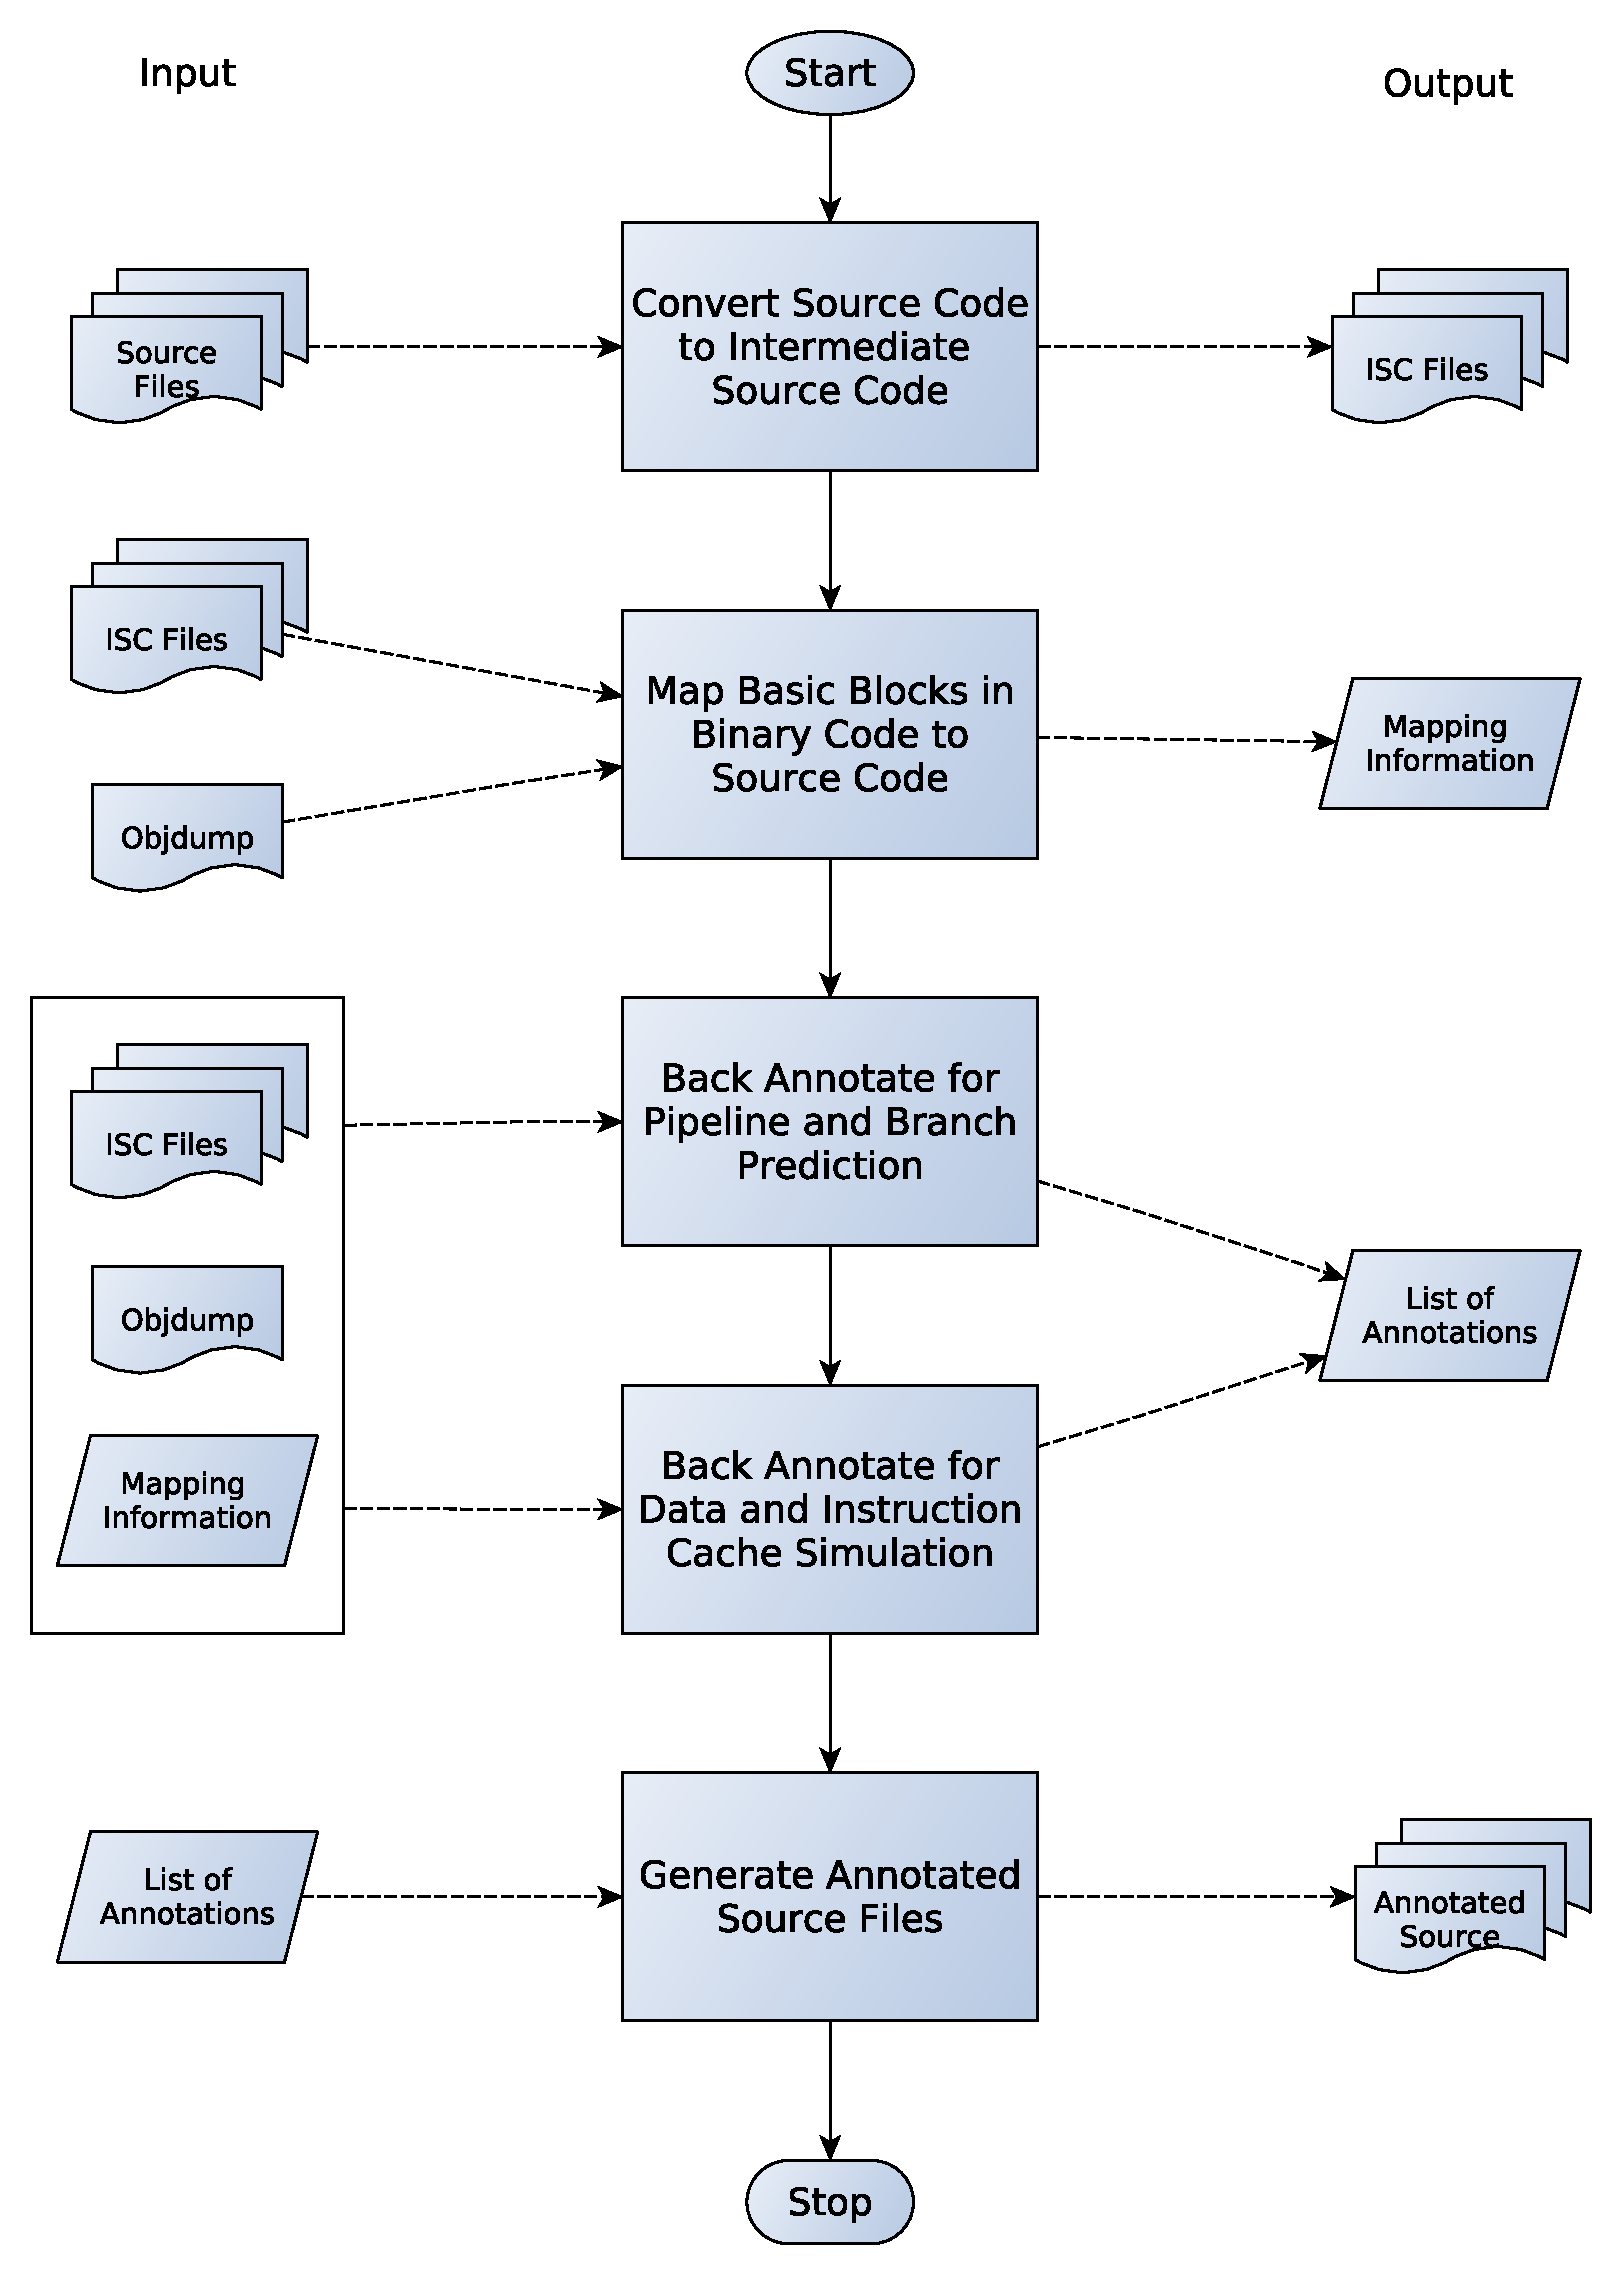
\includegraphics[width=.73\textwidth]{figures/HCS_FlowChart.pdf}
\caption{Flow Chart}
\label{fig:hcsFlowChart}
\end{figure}

%In this section, a brief overview of the project architecture is provided. Each part of the project is independent, and has been treated as a separate problem. The flow chart in figure [TODO] shows each step of the project. The approach to solve these techniques is presented in the subsequent sections in this chapter. Details of the implementation have been presented in the next chapter.

%From the example, it is clear that for correctly instrumenting the code accurate mapping is required between the source code and the binary code. However, this mapping is usually destroyed during the optimization phases of the compiler. The first problem that is solved in this project is to generate accurate mapping information at the Basic Block granularity. 
%
%In the next step, GDB is used to derive information about each variable that is used in the application. During compiler optimization, most of the variables defined by the user are optimized out, hence this information can only be extracted from the debug information with the binary code. Names, addresses and sizes of Global and Local Variables are extracted.
%
%For simulating data cache, each load and store instruction is accurately matched to an instruction in the source code. The variable being accessed is identified, and the annotation to simulate the memory access is added to the code. For simulating the instruction cache, annotation is added for each basic block in the binary code to the corresponding basic block in the source code.
%
%To estimate the amount of cycles spent in execution of a basic block in the processor pipeline, each instruction in a basic block is sequentially parsed to identify interlocking. Interlocking occurs when there is a Control or Data Dependency between instructions, which results in pipeline stall for a few cycles. The cycles used by each basic block are annotated back to the code. Further, a mechanism to emulate Branch Prediction Unit has been implemented. 

\section{Source Code to Intermediate Source Code}
From the example, it is clear that accurate mapping between source code and binary code is very important for instrumentation. Unfortunately, this mapping is destroyed during the optimization phases of the compiler. Extracting accurate mapping information is a challenging problem. In this project, an approach recommended in \cite{RBA2013} has been used to reduce the complexity of this problem.

The compiler performs these optimizations in two stages. The front-end of the compiler, translates the source code from a high-level language like C, to an Intermediate Representation (IR) called GIMPLE. The processor independent optimization strategies are applied in the front-end. In the back-end of the compiler, the optimized IR code is translated into Machine Language for the target processor. The processor dependent optimization strategies are applied in this phase.

The optimized IR Code has a control flow similar to that of the Binary Code, since front-end optimization strategies have already been applied. It should be comparatively easier to perform mapping between the IR Code and the Binary Code. However, instrumentation of IR Code is difficult as it is in the GIMPLE format. 

In this project, the source code of the benchmark application is cross-compiled, and the optimized IR Code is translated back into a high-level language, C. The generated code is called \gls{isc}. The code to convert GIMPLE code to C code has been reused from \cite{RBA2013}.

\begin{figure}[h]
\centering
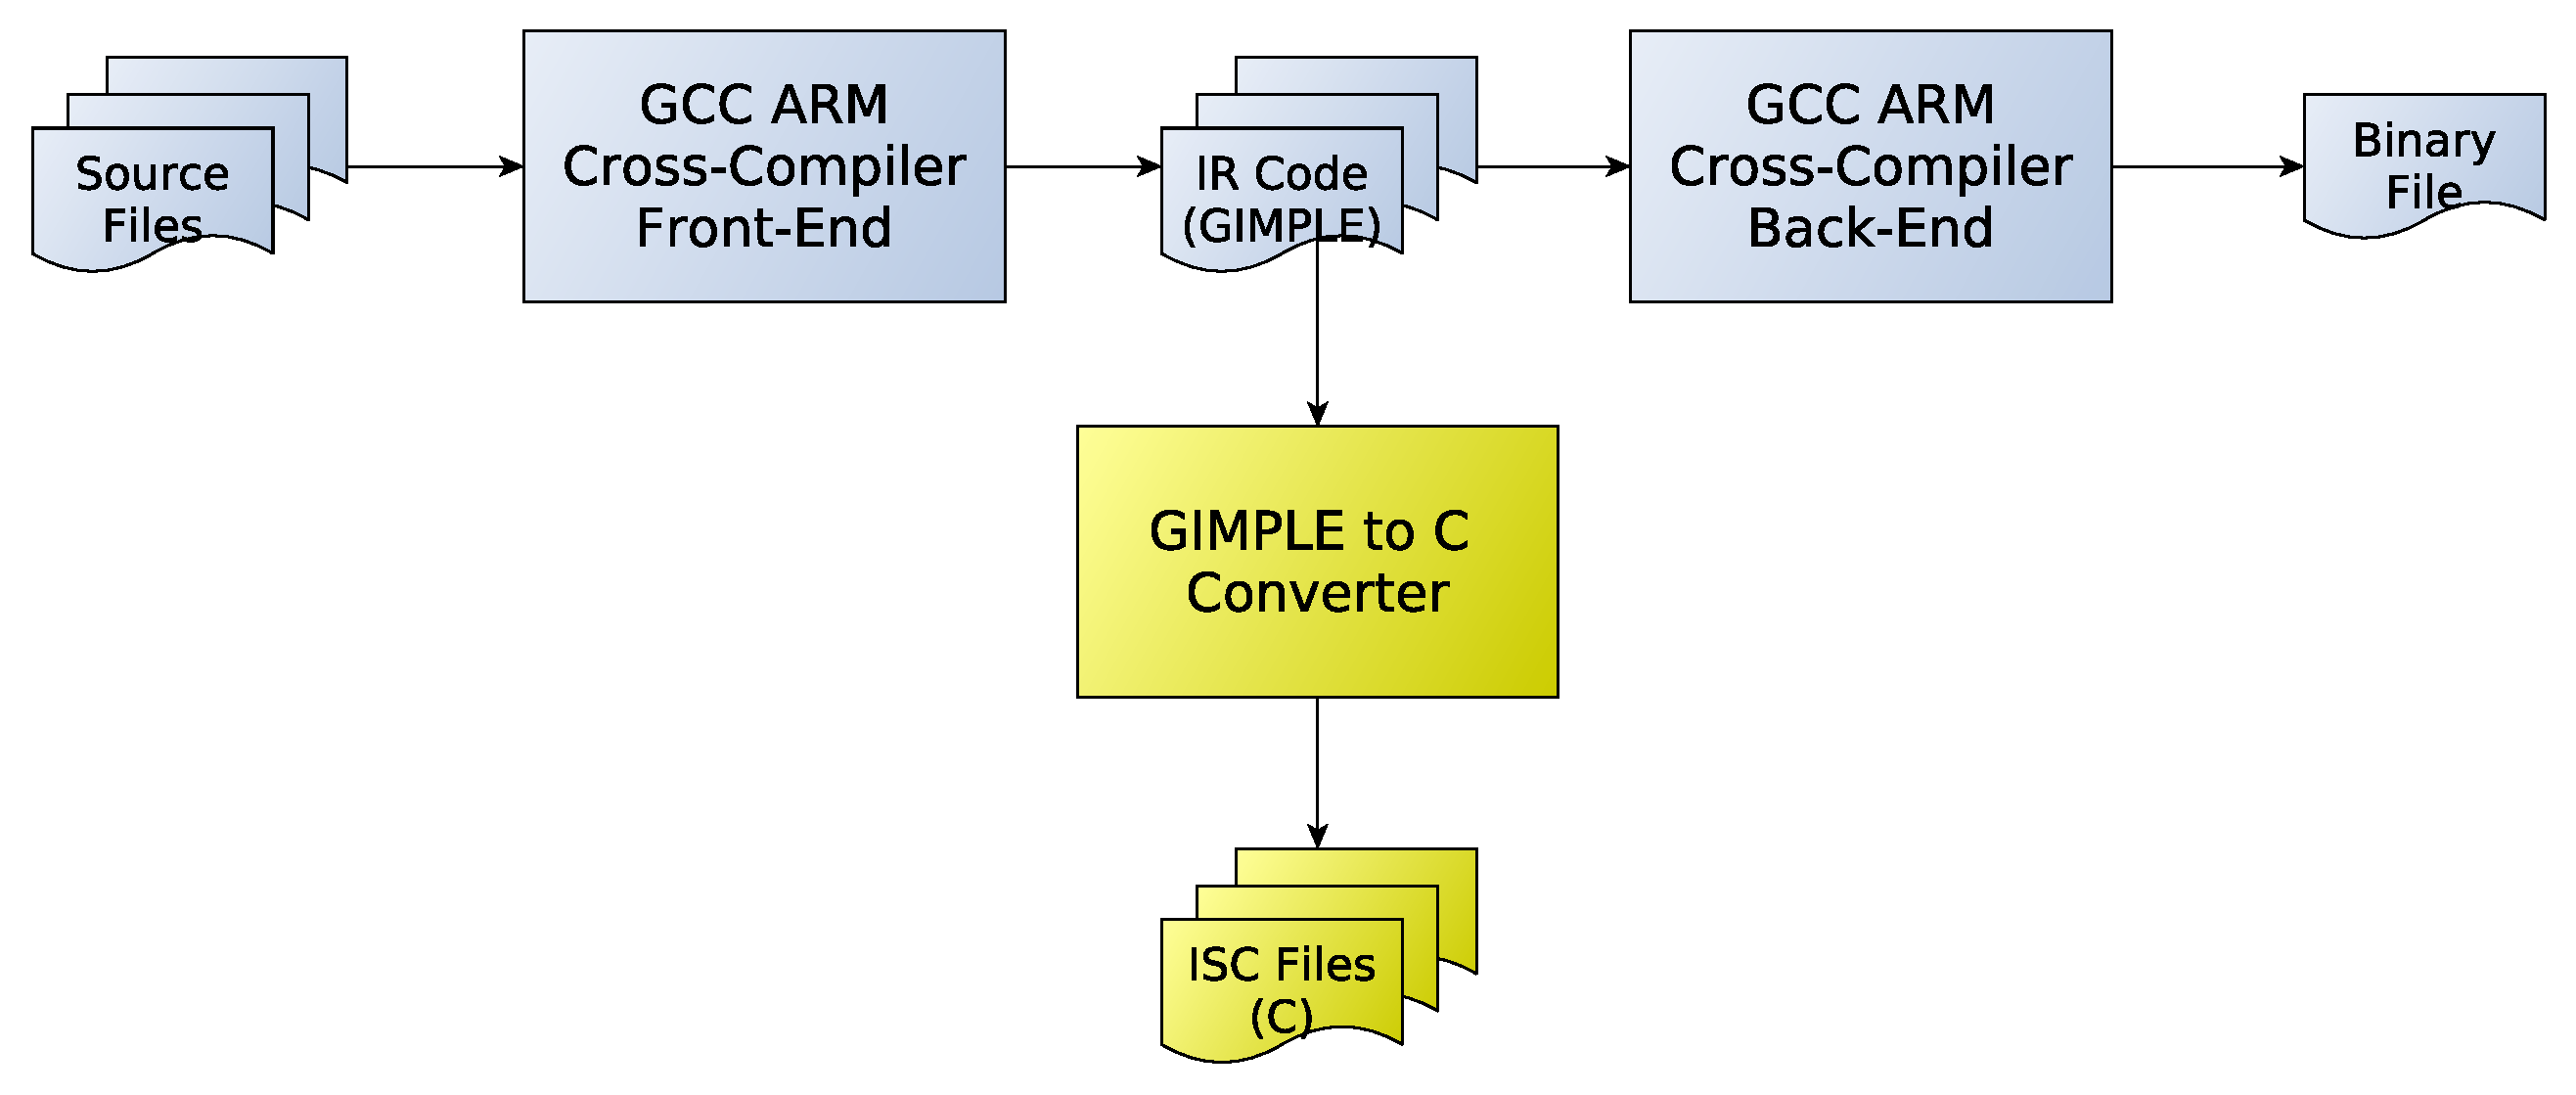
\includegraphics[width=.9\textwidth]{figures/ir2cConversion.pdf}
\caption{Conversion of Source Code to Intermediate Source Code}
\label{fig:ir2cConversion}
\end{figure}

Extracting mapping between \gls{isc} and binary code is comparatively easier. This is aided by the fact that \gls{isc} is easier to parse, as it uses simple \emph{if-else} constructs and \emph{goto} commands to implements loops. \gls{isc} is fairly easy to read and understand for the developer. Instrumentation is performed to the \gls{isc}. 

To aid understanding, the ISC will be interchangeably referred to as the source code in further sections.

A sample of ISC code generated by the tool is shown in Appendix \ref{app:ir2cConversion}.

\section{Mapping between ISC and Binary Code}
Even between \gls{isc} and Binary Code, the control flow is significantly different. This is because processor dependent optimizations are not included in the ISC. Modern processors offer complex optimization features. These features are processor-dependent and can only be utilized by the compiler back-end.

Compiler optimizes code by moving instructions around. New basic blocks may be created and some blocks may get merged in the binary code. A complete one to one mapping between basic blocks may often not exist. The mapping algorithm must take this into account, and find a mapping such that each basic block in the binary code maps to one or many basic blocks in the source code.

GDB can be used to extract mapping between instructions in binary code and statements in the source code. However, this mapping was observed to be highly inaccurate. To perform accurate mapping, complex techniques have been proposed based on analysis of Data and Control Flow. In this project, the Control Flow Graphs (CFGs)\footnote{Control Flow Graph is a graph representing flow of control among basic blocks in the code. The nodes represent basic blocks, and the edges represent the possible flow of execution.} of \gls{isc} and binary code are analysed using a mapping algorithm. The approach is inspired from \cite{RBA2013}. The mapping algorithm is based on the standard Graph Matching Algorithm using recursive Depth First Traversal.

%\begin{wrapfigure}{hrt}{0.4\textwidth}
%\vspace{-30pt}
%\begin{center}
%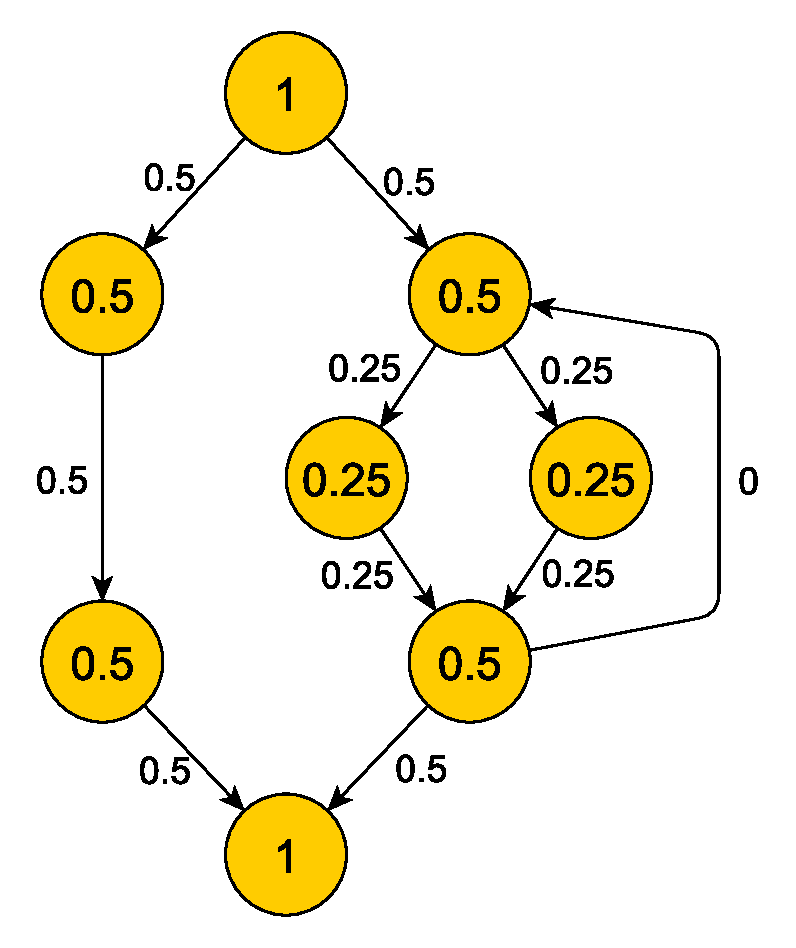
\includegraphics[width=.35\textwidth]{figures/flowValueComputation.pdf}
%\end{center}
%\vspace{-20pt}
%\caption{Computation of Flow Value}
%\vspace{-20pt}
%\label{fig:flowValueComp}
%\end{wrapfigure}

\begin{figure}[h]
\centering
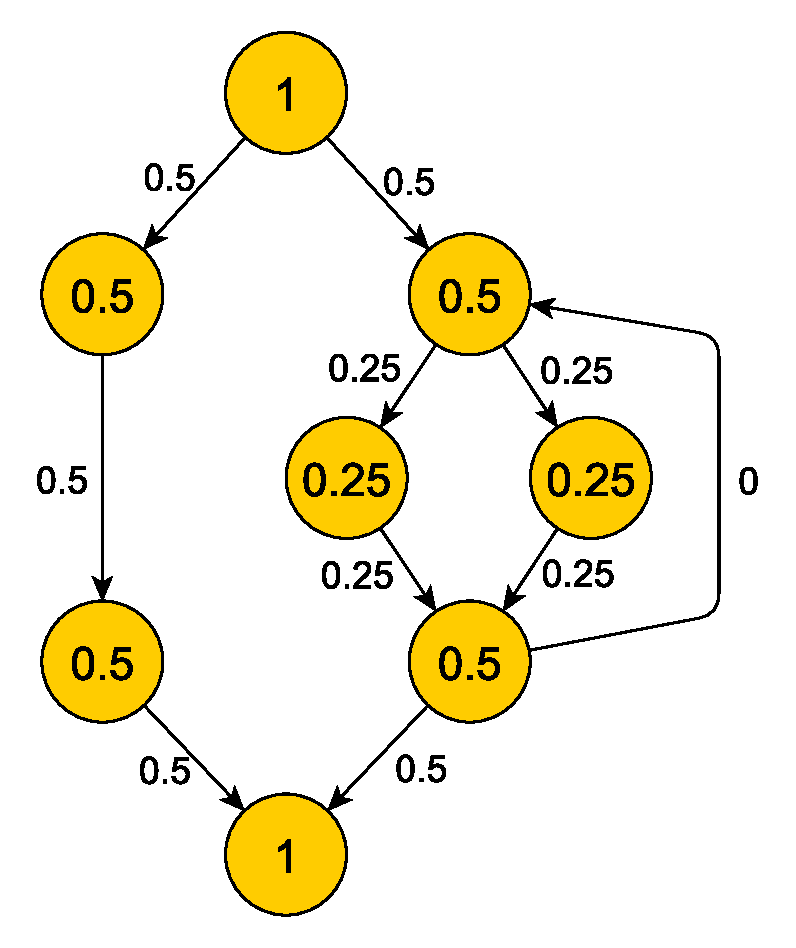
\includegraphics[width=.35\textwidth]{figures/flowValueComputation.pdf}
\caption{Computation of Flow Value}
\label{fig:flowValueComp}
\end{figure}

CFGs are extracted by parsing the source code and the binary code. To assist in mapping, a \textit{flow} value is calculated for each node in the graphs. The \textit{flow} value for a node is the sum of the \textit{flows} of the incoming edges to the node, which in turn is equally divided among the outgoing edges to successor nodes. \textit{Flow} for backward edges is 0. The \textit{flow} value of the root node is 1. Only nodes with equal flow value can be mapped to each other. Figure \ref{fig:flowValueComp} shows the computation of flow value in a graph. The labels on the nodes and edges represent the flow value.

The pseudo code of the \emph{mapping} function is presented in Algorithm \ref{algo:mapping}. The recursive function takes two nodes as parameter, and tries to find if the nodes map to each other. It checks that the nodes have the same \textit{flow} values, and returns \textit{False} if not. If the nodes have already been mapped to each other, the function returns \textit{True}. 

% http://tex.stackexchange.com/questions/163768/write-pseudo-code-in-latex
% TODO Complete algorithm
\begin{algorithm}[h!]
\caption{CFG Mapping Algorithm}\label{algo:mapping}
\begin{algorithmic}[1]
\Function{Mapping}{BB\_src, BB\_bin}
\If {\textit{flow}(BB\_src) != \textit{flow}(BB\_bin)}
\State \Return false
\EndIf
\\
\If {(BB\_src, BB\_bin) $\in$ MappingDict}
\State \Return true
\EndIf
\\
\State // Check for effects due to Compiler Optimization here
\\
\State SS\_src = \textit{Succ}(BB\_src)
\State SS\_bin = \textit{Succ}(BB\_bin)
\If {\textit{len}(SS\_src) != \textit{len}(SS\_bin)} 
\State \Return False
\EndIf
\\
\For {S\_src in SS\_src}
\For {S\_bin in SS\_bin}
\If {\textit{Mapping}(S\_src, S\_bin) == True}
\State break
\Else
\State continue
\EndIf
\EndFor
\State // Mapping could not be found for S\_src
\State \Return false
\EndFor
\\
\State // All children mapped; Input Nodes must map to each other
\State MappingDict $\leftarrow$ (BB\_src, BB\_bin)
\State \Return true
\\
\EndFunction
\end{algorithmic}
\end{algorithm}

At this point, special handling for different compiler optimizations is done. Section \ref{subsec:CondExec} illustrates the handling for Conditional Execution optimization that is frequently seen in the test set of benchmarks.

Hereafter, the successor sets of both nodes are created. Two nodes can be mapped to each other, only if they have the same number of successor nodes. For each successor \emph{S\_src} in \emph{SS\_src}, a matching node in \emph{SS\_bin} is identified by recursively calling the \emph{mapping} function. 

The nodes map to each other, if a mapping can be found for all successor nodes. The algorithm tries to find matching path from the start node, to the exit node and creates mapping between the nodes on this path.

The mapping algorithm has limitations. For instance, it can not differentiate between the \emph{then} and the \emph{else} block in an \emph{if-then-else} construct. Mapping from GDB is used to resolve such situations.

The mapping algorithm might fail in some corner cases. For the benchmark applications used for testing, the algorithm was found to work accurately.
The instrumentation tool generates graphical representation of the mapping between the CFGs. Users can easily verify the accuracy of mapping by analysing this output.

Mappings generated for some benchmark applications that were used for testing have been shown in Appendix \ref{app:mappingAlgo}.

\subsection{Handling of Conditional Execution Optimization}
\label{subsec:CondExec}

%TODO: Should this be moved to appendix?

Conditional Execution or Branch Predication is a feature supported in some Instruction Set Architectures to mitigate the cost associated with conditional branching. Consider the following example to understand the performance impact of this feature.

Example \ref{ex:cIfElse} shows a simple \emph{if-then-else} construct written in C. The code checks if \emph{a} is greater than \emph{b}. If true, the value of \emph{a} is assigned to \emph{max}, else the value of \emph{b} is assigned to \emph{max}. Example \ref{ex:objIfElse} is representative of how the assembly code may look like without any optimization.

\begin{Example}[h]
\begin{lstlisting}
int max(int a, int b)
{
    int ret;
    if (a > b)
        max = a;
    else
        max = b;
    return ret;
}
\end{lstlisting}
\caption{Example C Code}
\label{ex:cIfElse}
\end{Example}

\begin{Example}[h]
\begin{lstlisting}
00008068 <max>:
    8068:       cmp     r1, r0
    806c:       blt     8078   
    8070:       mov     r0, r1
    8074:       b       807c
    8078:       mov     r0, r0
    807c:       bx      lr
\end{lstlisting}
\caption{Unoptimized Object Code}
\label{ex:objIfElse}
\end{Example}

Instructions take more than one cycle to execute. To improve throughput, execution unit in almost all processors is implemented as a multi-stage pipeline. Instructions are fed into the pipeline and executed in parallel.

The \emph{cmp} instruction on line 2 in Example \ref{ex:objIfElse} is fetched by the first stage of the pipeline. While it is being decoded in the next stage of the pipeline, the branch instruction on line 3 has been fetched. Depending on the result of the compare instruction, the branch will be taken or not taken. The result of the compare instruction has not yet been evaluated. The processor cannot know with certainty which instruction to fetch after the branch instruction.

By assuming that the branch will not be taken, the processor fetches the \emph{mov} instruction on line 4. If the prediction is incorrect the pipeline must be flushed and \emph{mov} instruction on line 6 must be executed next. The pipeline flush leads to loss of multiple clock cycles.

This loss can be reduced by using Conditional Execution, when supported by the architecture. Each instruction can be predicated with a condition. The instruction is executed in the pipeline, but the result is only written back (or committed) if the condition evaluates to true. In the optimized code in Example \ref{ex:objOptimizedIfElse} the \emph{movge} instruction will be executed, but the value of \emph{r1} will be written to \emph{r0} only if the result of the compare instruction is "Greater than" or "Equal". A few clock cycles can be saved if the length of the conditionally executed block is small.

\begin{Example}[h]
\begin{lstlisting}
00008068 <max>:
    8068:       cmp     r1, r0
    806c:       movge   r0, r1
    8070:       movlt   r0, r0
    8074:       bx      lr
\end{lstlisting}
\caption{Optimized Object Code}
\label{ex:objOptimizedIfElse}
\end{Example}

\begin{figure}[h!]
\centering
\begin{subfigure}[t]{.33\textwidth}
\captionsetup{margin=10pt}
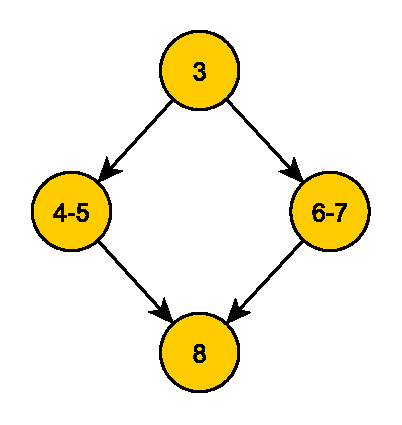
\includegraphics[width=\textwidth]{figures/CondExecSrcFlowChart.pdf}
\caption{Source Code}
\label{fig:cfgSrc}
\end{subfigure}%
~
\begin{subfigure}[t]{.33\textwidth}
\captionsetup{margin=10pt}
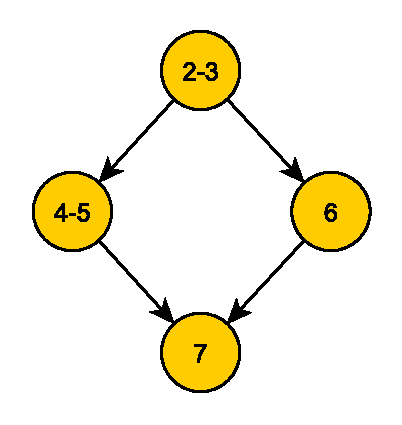
\includegraphics[width=\textwidth]{figures/CondExecObjUnoptFlowChart.pdf}
\caption{Unoptimized Binary Code}
\label{fig:cfgUnopt}
\end{subfigure}%
~
\begin{subfigure}[t]{.33\textwidth}
\centering
\captionsetup{margin=10pt}

\includegraphics[width=.5\textwidth]{figures/CondExecObjOptFlowChart.pdf}
\caption{Optimized Binary Code}
\label{fig:cfgOpt}
\end{subfigure}
\caption{Control Flow Graphs}
\end{figure}

The CFGs for the source code, and the unoptimized binary code have been represented in figures \ref{fig:cfgSrc} and \ref{fig:cfgUnopt}. The labels in the nodes represent line numbers for the corresponding basic blocks. These graphs are similar, and hence easy to map. However, in the optimized binary code the branching instructions are eliminated. The code is considered as a single basic block, as shown in the CFG in figure \ref{fig:cfgOpt}.

To handle this optimization, the binary basic block is analysed to check if Conditional Execution Instructions have been used. The corresponding basic block in source code must have a conditional branch, which can be identified by analysing the CFG. If the length of each conditional execution block in source code is smaller than a threshold, the algorithm predicts that the blocks have been merged using Conditional Execution. All four blocks in the source code are mapped to the single block in the binary code.

The mapping continues between the source code basic block after the \emph{if-then-else} construct, and the current binary basic block. If mapping is not found by this approach, the algorithm will recursively visit this step, and try another approach. 

\section{Annotation for Execution Cycles}
The estimation of number of cycles spent in execution of the instructions is done at a basic block granularity. Cycles spent in executing each basic block in binary code is estimated by static analysis. The cycles are annotated in the mapped basic block in the source code. Each time when the basic block is executed, the annotated cycles are accumulated in a global variable.

In the example in Section \ref{sec:SimpleExample}, a very simple processor was used where each instruction takes one cycle to execute. Estimation of cycles consumed in executing a set of instructions in such a processor is easy. In reality, each instruction takes multiple cycles to execute. To improve the throughput processors use a multi-stage pipelined execution unit. Each stage in the pipeline takes one cycle. The stages in a general pipelined execution unit are shown in Figure \ref{fig:genericPipeline}.

\begin{figure}[h]
\centering
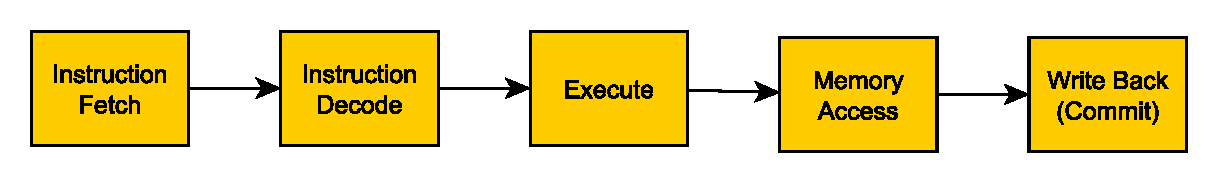
\includegraphics[width=\textwidth]{figures/genericPipeline}
\caption{Stages in a Pipelined Execution Unit}
\label{fig:genericPipeline}
\end{figure}

The first instruction is \textit{fetched} into the pipeline in the first stage. While this instruction is being \textit{decoded} in the next stage, the consecutively next instruction is \textit{fetched}. The \textit{execution} of the instruction is done in the third stage. The fourth stage is used for instructions that need to access memory, such as the load/store. The result of the execution is written back to the destination register in the final stage. In a best case scenario, the cycles consumed in execution of each basic block can be calculated as follows.

\begin{gather}\label{eq:2.1}
Cycles = n\_inst + n\_stages - 1
\intertext{where}
\begin{aligned}
n\_inst &= \text{Number of instructions in the basic block}\\
n\_stages &= \text{Number of stages in the pipeline}
\end{aligned} \notag
\end{gather}

However, consecutive instructions may have data and control dependency which will lead to stalling of the pipeline. Data dependency occurs when one instruction use the result generated by the previous instruction as an input. Refer to the example \ref{ex:dataDep}.  The result of the \emph{add} instruction will be written to \emph{r0} in the final stage in the pipeline. Meanwhile, the next instruction \emph{mul} needs the value of \emph{r0}. The execution of the \emph{mul} instruction will be stalled until, the result of the \emph{add} instruction has been written in \emph{r0}.

\begin{Example}
\begin{lstlisting}
806c:     ...
8070:     add     r0, r1, r2
8074:     mul     r3, r0, r4
8078:     ...
\end{lstlisting}
\caption{Illustration of Data Dependency among instructions}
\label{ex:dataDep}
\end{Example}

Some operations like floating point arithmetic, need more than one cycle to execute. The execution unit for such operations is implemented outside the pipeline. Control dependency occurs when an instruction needs a resource, which is being used by the previous instruction. Again, execution of the subsequent instruction is stalled until the resource is freed by the previous instruction.

To estimate the cycles spent in execution of a basic block, the structure of the pipeline and effects due to Data and Control Dependencies are taken into consideration. Instructions in each basic block are parsed sequentially, and dependencies are identified. The actual cycles spent in execution on the pipeline, are estimated by adding appropriate penalties for pipeline stalls to the equation \ref{eq:2.1}.

In this step, the latency in fetching data from the memory is ignored. This will be taken into account in section \ref{sec:AnnotMemAccess}. Also, it is assumed that the pipeline is empty at the beginning of each basic block. This may not be the case always, and will be considered in section \ref{subsec:BranchPred}.

The total number of cycles as calculated from the simulation is annotated to the corresponding basic block in the source code, as illustrated in Example \ref{ex:annotExecCycles}. On entering the basic block, global variable \emph{execCycles} is incremented by the number of cycles spent in executing the basic block. This is done each time the basic block gets executed.

\begin{Example}[h]
\begin{lstlisting}
unsigned long long execCycles = 0;

void foo()
{
    ...
    for(i=0; i<20; i++)
    {
        `execCycles += 24;` // Cycles spent in execution of this basic block
        ...
    }
    ...
}
\end{lstlisting}
\caption{Annotation for Execution Cycles}
\label{ex:annotExecCycles}
\end{Example}

\subsection{Branch Prediction}
\label{subsec:BranchPred}
To calculate the cycles spent in execution, it was assumed that the pipeline is empty at the beginning of each basic block. This may not always be the case and will be taken into account here.

\begin{Example}[h]
\begin{lstlisting}
806c:     ...
8070:     mov     r0, #0
8074:     ...
...
808c:     add     r0, #1
8090:     cmp     r0, #20
8094:     blt     8074
8098:     ...
\end{lstlisting}
\caption{Implementation of a loop using Conditional Branching Instructions}
\label{ex:condBranch}
\end{Example}

Conditional branching is implemented in binary code as a compare instruction followed by a conditional branch instruction. Example \ref{ex:condBranch} shows the implementation of a loop. The branch on line 7 is taken depending on the result of the compare instruction. In a pipelined execution unit, the result of the compare instruction may not be available in time to decide the instruction to be fetched after the branch instruction. The processor uses \gls{bpu} to predict the outcome of the branch instruction. The appropriate instructions are loaded into the pipeline.

If the prediction is incorrect, the pipeline must be flushed and the correct instruction to be executed next must be fetched. If the prediction is correct, a few cycles are saved. To account for the saved cycles, the \gls{bpu} is simulated.

The \gls{bpu}, uses heuristics to predict the outcome of a branch instruction. A state machine is implemented to predict the outcome of the branch. A table maintains the history of branch instructions seen in the recent past. The address of the branch instruction is stored along with a 2-bit state information. The states and transitions for each branch are shown in the state machine diagram in figure 
\ref{fig:bpuSMD}.

\begin{figure}[h]
\centering
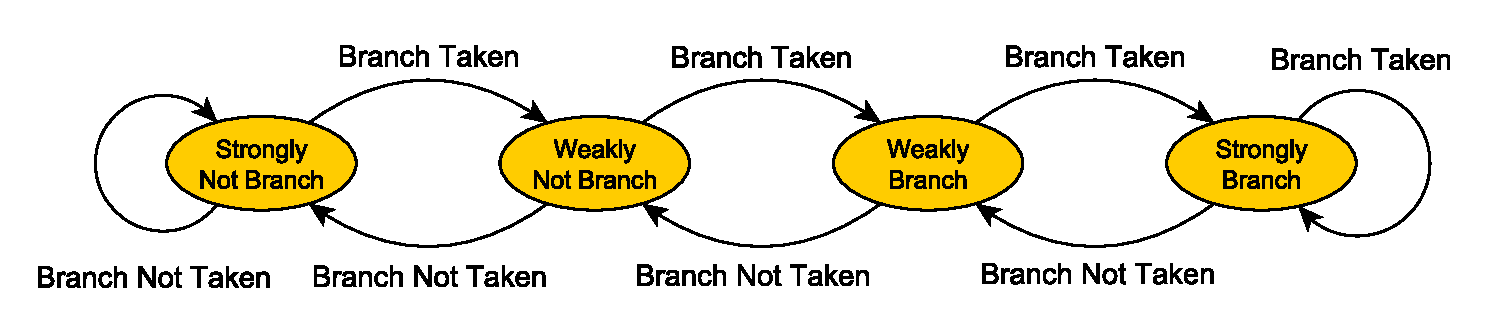
\includegraphics[width=\textwidth]{figures/BranchPredictionSMD.pdf}
\caption{State Machine Diagram implemented in the Branch Prediction Unit}
\label{fig:bpuSMD}
\end{figure}

The \gls{bpu} predicts that the branch will not be taken, when the current state is either "Strongly Not Branch" or "Weakly Not Branch". In the other states, the \gls{bpu} predicts that the branch will be taken.

When a branch instruction is loaded into the pipeline, the \gls{bpu} checks if the information for the branch is present in the history table. If an entry is not found, the processors predicts that the branch will not be taken. An entry is added to the table with state "Strongly Not Branch". When the branch is found in the history table, the prediction is made based upon the current state of the entry. The state of the entry is changed accordingly, when the outcome of the branch is known.

\begin{Snippet}[h!]
\begin{lstlisting}
/**
 * @brief Function to simulate Branch Prediction Algorithm.
 *
 * @param Start Address of the basic block
 * @param End Address of the basic block
 *
 * @return True, if branch was predicted
 *          False, if branch was not predicted
 */
unsigned int enterBlock(unsigned long startAddress,
                           unsigned long endAddress);
\end{lstlisting}
\caption{API offered by Branch Prediction Simulator}
\label{snip:branchPredAPI}
\end{Snippet}

A Branch Prediction Simulator has been developed which uses the same algorithm. It offers the API as shown in Snippet \ref{snip:branchPredAPI}. 

The function is called at the beginning of each basic block. The start and end address of the basic block is passed as a parameter to the simulator. This information is extracted from the binary code. The simulator checks whether the branch from the previous block to current block would have been predicted by the \gls{bpu}. It returns \emph{True} if the branch would have been predicted correctly, in which case a few cycles are subtracted from \emph{execCycles}. The instrumentation is done as shown in Example \ref{ex:branchPred}.

\begin{Example}[h!]
\begin{lstlisting}
unsigned long long execCycles = 0;

void foo()
{
    ...
    for(i=0; i<20; i++)
    {
        `execCycles += 24;` // Cycles spent in execution of this basic block
        `execCycles -= (enterBlock(0x8040, 0x8080) ? 4 : 0);`
        ...
    }
    ...
}
\end{lstlisting}
\caption{Instrumentation for simulating Branch Prediction Unit}
\label{ex:branchPred}
\end{Example}

\section{Annotation for Memory Access}
\label{sec:AnnotMemAccess}
The cycles spent in fetching data and instructions from the memory must be accurately estimated. To do this a Cache Simulator has been implemented. The source code is instrumented to invoke the Cache Simulator at run-time. In the following sections details about the Cache Simulator have been discussed, followed by the process to instrument the code.

\subsection{Cache Simulator}
Most processors use a hierarchy of low-latency cache memories to improve performance by reducing the time spent in fetching data from memory. Caching has a significant impact on performance. To take this into account, an accurate simulation of the cache hierarchy needs to be done.

The Cache Simulator emulates the caching hierarchy of the target processor. It keeps a track of the data stored in the caches. Whenever a memory access is performed, the simulator checks whether the data can be fetched from the caches. If the data is not found in any cache, it must be fetched from the memory. The simulator returns the number of cycles that would be spent in performing the memory access on the target processor.

\begin{Snippet}[h!]
\begin{lstlisting}[numbers=none]
/**
 * @brief Function to simulate Data Cache Access.
 *
 * @param Address of the data to be fetched
 * @param True, if read access; False, if write access
 * @param Detailed result for trace
 *
 * @return Number of cycles spent in performing access.
 */
unsigned long long simDCache(unsigned long address,
                                unsigned int is_read_access,
                                struct csim_result_t *csim_result);
                                
/**
 * @brief Function to simulate Instruction Cache Access.
 *
 * @param Start Address of the basic block
 * @param Size of the basic block in Bytes
 * @param Detailed result for trace 
 *
 * @return Number of cycles spent in performing access.
 */
unsigned long long simICache(unsigned long address,
                                unsigned long size,
                                struct csim_result_t *csim_result);
\end{lstlisting}
\caption{API provided by Cache Simulator}
\label{snip:csimAPI}
\end{Snippet}

Most processors use separate cache for Data and Instructions. The cache simulator offers the API mentioned in snippet \ref{snip:csimAPI} to simulate different types of memory accesses.

For each data access in the application, annotation is done in the source code to call function \emph{simDCache} and trigger Data Cache simulation. The address of the data being fetched is provided as parameter, along with a flag to signify whether it is a read or write access. Simulation of Instruction Cache is done at basic block granularity. \emph{simICache} is called with the start address of the basic block and the size of the basic block in bytes as parameters. Number of cycles spent in performing the memory access is returned by the cache simulator. The return value from the cache simulator is accumulated in a global variable \emph{memAccessCycles}. 

\begin{Snippet}[h!]
\begin{lstlisting}[numbers=none]
struct csim_result_t
{
	unsigned long long L1Hits;
	unsigned long long L2Hits;
	unsigned long long L2Misses;
	unsigned long long prefetches;
};
\end{lstlisting}
\caption{Data Structure for storing detail statistics from Cache Simulator}
\label{snip:csimAPI}
\end{Snippet}

In addition, the Cache Simulator provides detailed statistics. These results are stored by the Cache Simulator in an object of type \emph{struct csim\_result\_t}. The pointer to the object is passed to the Cache Simulator as the third parameter in the API. This data will be useful for estimating power consumption, as will be discussed later. 

The source code is instrumented, as illustrated in example \ref{ex:cacheSimGlobVar}, to create global variables to record the result of cache simulation.

\begin{Example}[h!]
\begin{lstlisting}
unsigned long long execCycles = 0;
`unsigned long long memAccessCycles = 0;`
`struct csim_result_t csim_result;`

void foo()
{
    ...
\end{lstlisting}
\caption{Global Variables declared for results from Cache Simulation}
\label{ex:cacheSimGlobVar}
\end{Example}

\pagebreak
\subsubsection{Cache Features and Parameters}

Caches may have varying parameters and features such as,
\begin{itemize} \itemsep -2pt
\item Sizes
\item Approach for Associativity of Data (Direct Mapped, N-way Set Associative)
\item Hierarchy (multiple levels of caching)
\item Replacement Policies
\item Data Prefetching Policies
\end{itemize}

The cache simulator has been designed in a modular fashion. Platform specific implementation of the cache may be plugged into the API. Architects can alter specific parameters of the cache like size and associativity to analyse the impact on performance, without having to instrument the code again.

Details about the hierarchy and features that have been implemented in the Cache Simulator to model the target processor used for testing have been discussed in Section \ref{sec:c3CacheHierarchy}.

\section{Instrumentation for Instruction Access}
For estimating cycles spent in fetching the instructions from memory, instrumentation is performed at the basic block granularity. 

For each basic block in the cross-compiled binary code, the address of the first instruction in the block and size of the block in bytes is extracted by static analysis. Note that since the binary is compiled to be run on Bare-Metal, the load address of the binary was decided at compile time. The addresses of instructions extracted from the binary, are the physical addresses where the instructions will reside in the memory of the target system.

The corresponding basic block in the source code is identified from the mapping information. Instrumentation is performed at the beginning of the basic block, and the instruction access is simulated using the API provided by the cache simulator. The instrumentation is illustrated in Example \ref{ex:instCacheInst}.

\vspace*{10pt}
\begin{Example}[h!]
\begin{lstlisting}
unsigned long long execCycles = 0;
unsigned long long memAccessCycles = 0;
struct csim_result_t csim_result;

void foo()
{
    ...
    for(i=0; i<20; i++)
    {
        execCycles += 24; // Cycles spent in execution of this basic block
        execCycles -= (enterBlock(0x8040, 0x8080) ? 4 : 0);
        `memAccessCycles += simICache(0x8040, 32, &csim_result);`
        ...
    }
    ...
}
\end{lstlisting}
\caption{Instrumentation for simulating Branch Prediction Unit}
\label{ex:instCacheInst}
\end{Example}

\section{Instrumentation for Data Access}
The instrumentation in the example shown in Section \ref{sec:SimpleExample} was simplified for illustration. It had a flaw which will result in inaccuracy of estimation. To simulate load operation for fetching elements of \emph{array}, the address of \emph{array} from the Host Machine was used. For accurate estimation, data access must be simulated using target addresses. This is important since the host and target memory systems may vary significantly. 

For instance, the host and target system may use different sizes for basic data types. The host machine in our test setup uses 8 Bytes for \emph{long int} and the target machine uses 4 Bytes for the same data type. When accessing elements of an array of \emph{long int}s using host addresses, twice the number of cache-misses will be reported than what is expected on the target device.

The address for each load/store instruction needs to be resolved for the target processor. This can not be done by static analysis. The technique to do this is inspired from research published in \cite{Lu2013} and is called Memory Access Reconstruction. 

Multiple steps are involved in this process. These steps are described in the following sections.

%The steps needed for Memory Access Reconstruction are as follows
%
%\begin{itemize} \itemsep -6pt
%\item Extract address of each variable used in the program.
%\item Analyse binary code for identifying load/store operations on variables.
%\item Parse the source code to identify and analyse statements causing the access.
%\item Perform Instrumentation
%\end{itemize}

\subsection{Resolve address of each variable}
The address of each variable used in the program is extracted. This information is useful in later steps. A program may use different types of variables. The technique to resolve the address of each type of variable has been described in this section.

\subsubsection{Global Variables}
Global Variables are accessible by all functions, and are stored in the Data Section of the application memory. The physical addresses of the global variables are decided at compile time. The address, size and type of each Global Variable is extracted by static analysis of the binary using GDB. 

For each global variable \emph{var}, another global variable \emph{var\_addr} is declared by instrumentation. The address of the global variable on the target system is stored in this variable. This address is later used for simulating access to the global variable. Refer to the example \ref{ex:GlobVarInst}.

\vspace*{10pt}
\begin{Example}
\begin{lstlisting}
int globalVar[20];
`unsigned long globalVar_addr = 0x7c8;` // Address of global variable

void foo ()
{
    ...
}
\end{lstlisting}
\caption{Instrumentation to resolve address of Global Variables on Target Device}
\label{ex:GlobVarInst}
\end{Example}

\subsubsection{Local Variables}
Local Variables are defined inside a function definition, and are only accessible inside the function. Memory for local variables is only allocated when the function is called, and is located in the stack frame of the function. The actual physical address of the local variables can not be resolved by static analysis, as the stack grows and compacts at run-time. However, the address of each local variable relative to the value of the stack pointer, can be known.

\begin{Example}[h]
\begin{lstlisting}[label=lst:LocalVarInst]
`unsigned long CSIM_SP = 0x1ff28;` // Intial Value of Stack Pointer

void foo ()
{
    double localVar;
    `unsigned long localVar_addr = 0x08;` // Address relative to SP

    `CSIM_SP = CSIM_SP + 0x16;` // Increment by size of stack frame
    
    ...
    
    `CSIM_SP = CSIM_SP - 0x16;` // Decrement by size of stack frame
    
    return;
}
\end{lstlisting}
\caption{Instrumentation to resolve address of Local Variables on Target Device}
\label{ex:LocalVarInst}
\end{Example}

If the value of the stack pointer is known, the relative address can be added to it to resolve the physical address of the local variable. Instrumentation is done to keep a track of the Stack Pointer, as shown in Example \ref{ex:LocalVarInst}. A global variable \emph{CSIM\_SP} is declared and initialized with the initial value of the stack pointer. The size of stack frame for each function is extracted by static analysis of the binary. The value of \emph{CSIM\_SP} is incremented at the beginning of each function by the size of the stack frame of the function, and decremented before the function returns.

The relative address of a local variable is also annotated in the code. The physical address of the variable at run-time is calculated by adding the relative address to the value of \emph{CSIM\_SP}.

\subsubsection{Dynamically Allocated Memory}
Dynamically Allocated Memory is stored in the Heap Section. To allocate and free heap memory, the application uses API provided by system libraries. The memory allocation algorithm of the target system needs to be emulated at run-time of simulation, to resolve physical addresses of dynamically allocated memory. This approach is discussed in \cite{Lu2013}. However, this is complicated to achieve, and has been ignored for this project. Only benchmark applications that do not use Dynamically Allocated Memory can be used. The project can later be extended to include this functionality.

\subsection{Analyse binary code for identifying load/store operations on variables}
\label{subsec:analyseBinary}
To identify which variable is being accessed, the binary code is partially simulated. A simple functional simulator is developed in Python, which maintains the state of each register in the target processor. Starting from the main function, each instruction in the binary code is parsed and state of the registers is updated. In this simulation, the branching instructions are ignored. This means, each instruction will only be parsed once. 

When a function is called, the state of the registers is stored and will be used as the initial state when simulating the function. This is done to keep track of function parameters sent as values in registers. When parameters are sent in the stack, this approach will fail. Each function is simulated once and subsequent calls to the function are ignored.

%\vspace*{-20pt}
\begin{figure}[h!]
\centering
\includegraphics[width=\textwidth]{figures/ParitalSimulator.png}
\vspace*{-20pt}
\caption{Illustration of the Partial Functional Simulator used to extract address of each load/store instruction in the binary code}
\label{fig:partialSimulator}
\end{figure}

The illustration in Figure \ref{fig:partialSimulator} shows how this works. The code from the simple example in Section \ref{sec:SimpleExample} has been used for illustration. The binary code of the \emph{sum} function is shown on the left. On the right, the symbol table shows the address of the global variable, \emph{globVar}. 

The state of the registers is shown when the function was called. Address of the \emph{globVar} was sent as a parameter to the function in register \emph{r0}. The values in the rest of the registers are arbitrary. The state of the registers is updated after parsing each instruction in the code. On line 4, a load instruction is seen. The address in \emph{r0} is indexed by the value in \emph{r3}, and the data is read into \emph{r1}. The address belongs to global variable \emph{globVar}. 

By doing this simulation, the address of each load/store instruction can be extracted. This information helps in identifying which variable is being accessed by the load/store instruction. 

\begin{itemize}
\item If the address belongs to Data Section, the instruction must be accessing a Global or Static Variable. Addresses of Global and Static Variables were extracted in the previous stage. The variable being accessed can be identified. 
\item If the address belongs to the Stack Space, it could be accessing a local variable. The variable being accessed is again identified from the information collected in the previous phase. Additionally, the stack space is used for register spilling. The load/store instruction could be associated with this operation. This can be distinctively identified, if no local variable is located on this address.
\end{itemize}

The memory accesses performed in each basic block in the binary code are recorded. Instrumentation for simulating these accesses will be done in the corresponding basic blocks in the source code. 

This approach has certain limitations. It may fail, in the presence of some pointer dereferencing operations. When the variable being accessed by a load/store instruction is not identified, appropriate hints are provided in the log to enable the user of the tool to manually instrument the code.

\subsection{Parse Source Code}
In the previous step, load/store instructions for register spilling were distinctly identified. Instrumentation for register spilling is straight-forward. For each load/store instruction corresponding to register spilling in a binary basic block, data cache access is simulated in the mapped basic block in the source code.

However, instrumentation of load/store instruction for variables is a more complicated. Note, that in the previous step only the variable being accessed by each load/store instruction were identified. In the example shown above \emph{globVar} is an array of integers. Elements of the array are accessed in a loop by adding an index to the base address of the array. To correctly instrument the Data Cache Access, the index must be known. This information can only be extracted by parsing the source code.

\begin{figure}[h]
\centering
\includegraphics[width=.5\textwidth]{figures/cParser.png}
\caption{Block Diagram for a custom C parser, that parses a statement and returns information about each variable accessed in the statement.}
\label{fig:customCParser}
\end{figure}

In this stage, the focus is to identify the statement in source code which causes memory access. By parsing this statement, additional information will be extracted to accurately instrument the code. A custom C Parser is implemented in Python to parse the Instrumented Source Code (ISC). Conversion of source code to ISC helps here, because ISC is easier to parse. The parser returns a list of variables being accessed by the statement, along with other information like index expression and whether it is a read or write operation. Refer to figure \ref{fig:customCParser}.

For each basic block in binary code, the mapped basic block in the source code is parsed. One to one mapping between each load/store operation and a statement in the source code is extracted. Annotation for the data access is performed. 

%\vspace*{10pt}
\begin{Example}[h]
\begin{lstlisting}
unsigned long CSIM_SP = 0x1ff28; // Initial Value of SP

unsigned long long memAccessCycles = 0;
struct csim_result_t csim_result;

unsigned int globVar[20];
unsigned long long globVar_addr = 0x7c8; // Address of Global Variable

void foo()
{
    unsigned int localVar;
    unsigned long localVar_addr = 0x08; // Address relative to SP
    
    CSIM_SP = CSIM_SP + 0x16; // Increment by size of stack frame
    
    ...
    *@localVar += globVar[i];@*
    `memAccessCycles += simDCache(globVar_addr + i * sizeof(int),`
                                    `READ_ACCESS,`
                                    `&csim_result);`
    `memAccessCycles += simDCache(CSIM_SP + localVar_addr,`
                                    `WRITE_ACCESS,`
                                    `&csim_result);`
    ...
    
    CSIM_SP = CSIM_SP - 0x16; // Decrement by size of stack frame
    return;    
}        
\end{lstlisting}
\caption{Instrumentation for simulating Branch Prediction Unit}
\label{ex:dataCacheInst}
\end{Example}

Annotation for simulating access to a global variable is straight-forward. The index expression, if any, extracted from the source code is added to the base address of the global variable in the target processor. For local variables, the value of \emph{CSIM\_SP} is added to the relative address to extract the base address of the local variable. The index, if any, is then added to this base address. Example \ref{ex:dataCacheInst} shows instrumentation of a local and global variable. The highlighted statement on line 17, causes a read operation on an element of array \emph{globVar} and a write operation to \emph{localVar}. Appropriate instrumentation is shown between lines 18 and 23.

\subsubsection{Handling of pointers sent as function parameters}

In the simple example in Section \ref{sec:SimpleExample}, pointer to an array is passed as a parameter to the function. By simulating the binary code in Section \ref{subsec:analyseBinary}, access to global variable \emph{globVar} was identified. However, the function \emph{sum} may be called with a pointer to any other array. Special handling needs to be done for such cases, when pointers are sent as function parameters.

The approach used in this project, is to modify the signature of each function that takes pointers as arguments. For each pointer argument \emph{ptr}, a new argument is added \emph{ptr\_addr}. The calling function is accordingly modified, to provide address of the variable on the target processor. When \emph{ptr} is dereferenced, data cache access is simulated using \emph{ptr\_addr}. 

TODO: Maybe we need another example here.

\section{Estimation of Power Consumption}
Apart from the speed of execution, the power consumption is a key performance indicator for modern processors. The balance between performance and power is critical, and needs to be maintained. An accurate estimate of power consumption can help architects keep this balance in check.

The approach to estimate the power consumption is inspired from [TODO]. The power consumption of processors mainly comes from dynamic power consumption due to switching activity and static power consumption due to the leakage current. This power consumption can be attributed to various components in the processor. These components are in active or idle state, depending on the operations being performed. In idle state, the power consumption is reduced as there is no switching activity. Through careful measurement, accurate estimation of dynamic and static power consumption of each component of the processor can be known.

The Dynamic Power Consumption of a system is a function of the Voltage and Frequency. It is derived by the following formula.

\begin{gather}
P = \alpha CV^{2}f 
\intertext{where}
\begin{aligned}
\alpha C &= \text{Equivalent Switching Capacitance of the circuit} \\
V &= \text{Supply Voltage} \\
f &= \text{Frequency}
\end{aligned} \notag
\end{gather}

The value of equivalent switching capacitance, $\alpha C$ can be measured for each component. Also, the frequency and supply voltage for each component is known. The Static Power Consumption for each component is constant, and can be measured.

%%TODO: keep always, check if image is aligned well.
%\begin{wrapfigure}{hrt}{0.3\textwidth}
%\vspace{-30pt}
%\begin{center}
%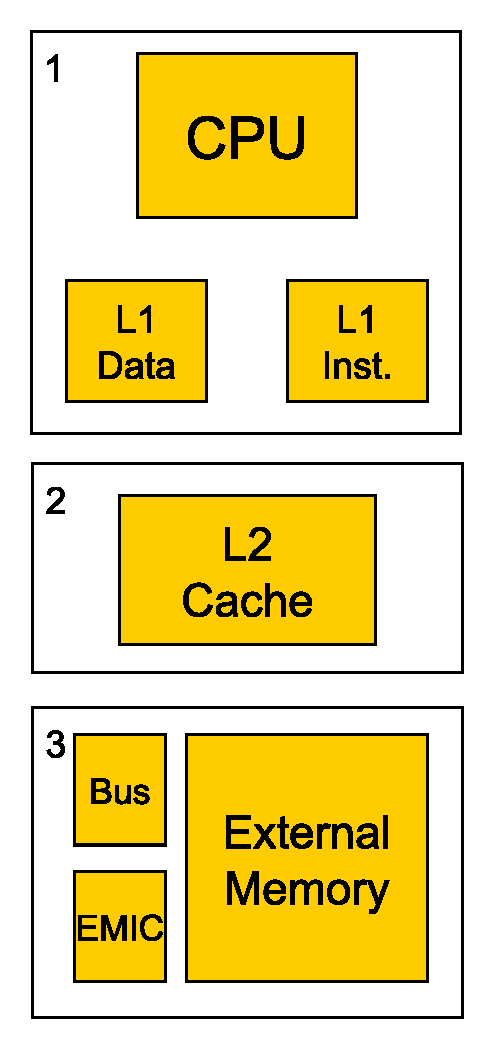
\includegraphics[width=.28\textwidth]{figures/components.pdf}
%\end{center}
%\vspace{-20pt}
%\caption{Components of a processor}
%\vspace{-20pt}
%\label{fig:components}
%\end{wrapfigure}

\begin{figure} [h]
\centering
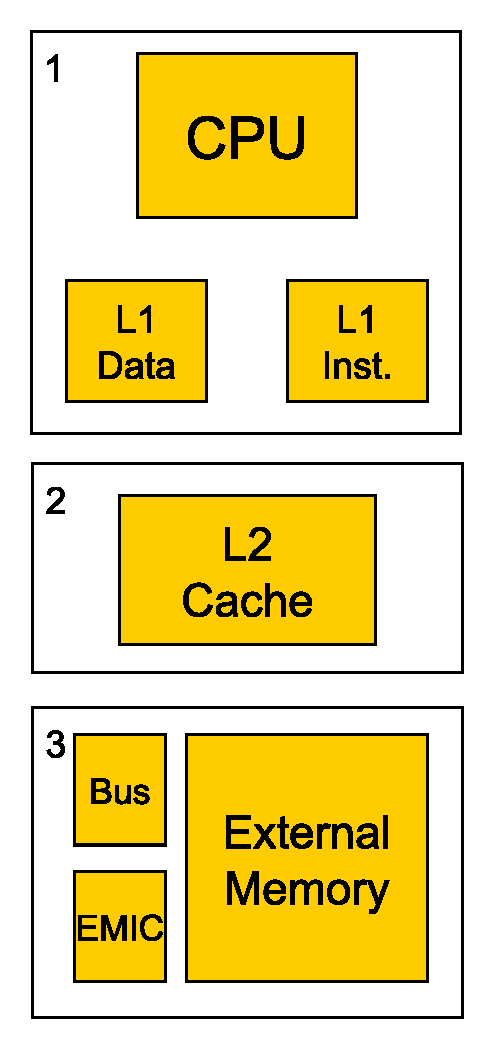
\includegraphics[width=.3\textwidth]{figures/components.pdf}
\caption{Components of a processor}
\label{fig:components}
\end{figure}

Some processors use Dynamic Voltage and Frequency Scaling technique to reduce the power consumption. Certain operating points are defined, and depending on the current load on the components the frequency and voltage is decided. The switching between operating points is handled by firmware, and can be disabled. This feature has not been considered in this project currently, however the approach can be extended to handle this feature effectively.

From information about state of each component at a point in time, the total power being consumed by the processor at that time can be estimated. This information can be extracted from the instrumentation performed in previous steps. An accurate model of components in the processor needs to be created. In this project, the processor has been divided into three components, as shown in Figure \ref{fig:components}

The CPU and the L1 Cache are collocated on a single die, and generally operate at the same frequency. They are grouped as a single component. This component is active when the instructions are being executed and L1 Miss does not occur. On L1 Miss, the L2 Cache is requested for data. The L2 Cache generally runs on a lower frequency, and is treated as a separate component. The L2 Cache is only active when an L1 Miss occurs. On L2 Miss, the data is fetched from the main memory. The main memory is generally located on an external chip. The memory is linked to the processor, generally though an External Memory Controller on a memory bus. The external memory, along with the interconnect is treated as a third component.

\subsection{Trace Collection}
Rather than average power consumption, it is interesting to see how the consumption changes over the time of execution of the application. In this project, the power consumption is estimated at the granularity of basic blocks. Using statistics generated from instrumentation performed previously, state of each component can be known over the time of execution of the basic block. The power consumed over the period of executing of this basic block can thus be calculated.

The CPU remains in switching state for \emph{execCycles} and in idle state for \emph{memAccessCycles}. Note, that when the data is fetched from L1 Cache, the CPU is not put idle state. Hence, grouping of L1 Cache with the CPU is justified. 

The Cache Simulator can tell whether the data was fetched from either of the caches or from the memory. The number of cycles spent in each access from L2 cache is constant. The L2 cache is in active state when an L1 Miss occurs. The data is looked up in the L2 cache. If data is not found, L2 Miss occurs and data is fetched from Memory. The memory is also in active state when data is prefetched by the processor. The Cache Simulator provides detailed statistics of number of L1 Hits, L2 Hits and L2 Misses and prefetches.

For estimating power consumption, this data is collected at the basic block graularity. The API provided by the Power Estimation Utility is shown in Snippet \ref{snip:pestAPI}

\vspace*{10pt}
\begin{Snippet}[h]
\begin{lstlisting}[numbers=none]
/**
 * @brief API to estimate the power
 *
 * @param Name of the current Basic Block
 * @param Number of cycles spent in active state of CPU
 * @param Number of cycles spent in fetching data from memory
 * @param Number of L2 Accesses = L2 Hits + L2 Misses
 * @param Number of memory accesses = L2 Misses + Prefetches
 *
 * @return Amount of Energy spent in the period of time in uJ.
 */
double estimate_power(unsigned long long execCycles,
                		unsigned long long memAccessCycles,
                		unsigned long long L2_Access,
                		unsigned long long memAccesses)
\end{lstlisting}
\caption{API provided by Power Estimation Utility}
\label{snip:pestAPI}
\end{Snippet}

The API is called at the end of each basic block. The current value of global variables \emph{execCycles} and \emph{memAccessCycles} is passed as parameter. The utility keeps track of previously reported cycles, and calculates the cycles spent in each activity in the current block. Similarly, the current value of sum of number of L2 Hits and number of L2 Misses is passed as the fourth parameter. Current value of sum of number of L2 Misses and number of prefetches is sent as the fifth parameter.

Using this data, the Power Estimation Utility calculates the total power consumed over this period. The data is written to an output file which can be plotted and analysed.

Example \ref{ex:powerEstInst} illustrates the instrumentation for estimating power consumption.

\vspace*{10pt}
\begin{Example}[h!]
\begin{lstlisting}
unsigned long long execCycles = 0;
unsigned long long memAccessCycles = 0;
struct csim_result_t csim_result;

void foo()
{
    ...
    for(i=0; i<20; i++)
    {
        ...
        `estimate_power(execCycles,`
                        `memAccessCycles,`
                        `csim_result.L2_Hits + csim_result.L2_Misses,`
                        `csim_result.L2_Misses + csim_result.prefetches);`

    }
    ...
}
\end{lstlisting}
\caption{Instrumentation for estimating Power Consumption}
\label{ex:powerEstInst}
\end{Example}
